\documentclass[10pt]{article} % page setup
\usepackage[margin=2cm]{geometry} % page setup
\usepackage{amsmath,amssymb,amsthm, mathtools} % helpful math cmds
\usepackage{graphicx} % for inserting images
\usepackage{enumitem} % enumerate config
\usepackage{footnote} % footnote fix
\usepackage{todonotes} % todos
\usepackage[colorlinks=true, allcolors=blue]{hyperref} % hypertext links
\usepackage{float}
\usepackage[numbers]{natbib}
\usepackage{caption}
\usepackage{subcaption}
\usepackage{gensymb}
\usepackage{listings} % typeset programs
\usepackage{blindtext} % placeholders
\usepackage{lastpage} % page references
\usepackage{fancyhdr} % header config
\usepackage{setspace} % line spacing
\usepackage{textcomp, gensymb} % additional symbols
\usepackage{parskip} % paragraph separation
\usepackage{cancel} % strikethroughs
\usepackage[T1]{fontenc}
\usepackage{physics}
\usepackage{pgfplots}
\usepackage{listings}
\usepackage{tikz}
\usetikzlibrary{positioning, arrows.meta}

\definecolor{codegreen}{rgb}{0,0.6,0}
\definecolor{codegray}{rgb}{0.5,0.5,0.5}
\definecolor{codepurple}{rgb}{0.58,0,0.82}
\definecolor{backcolour}{rgb}{0.95,0.95,0.92}

\lstdefinestyle{defaultstyle}{
  backgroundcolor=\color{backcolour},
  commentstyle=\color{codegreen},
  keywordstyle=\color{magenta},
  numberstyle=\tiny\color{codegray},
  stringstyle=\color{codepurple},
  basicstyle=\ttfamily\footnotesize,
  breakatwhitespace=false,
  breaklines=true,
  captionpos=b,
  keepspaces=true,
  numbers=left,
  numbersep=5pt,
  showspaces=false,
  showstringspaces=false,
  showtabs=false,
  tabsize=2
}
\lstset{style=defaultstyle}
\pgfplotsset{compat=1.18}
\renewcommand{\familydefault}{\sfdefault}

\newcommand{\documentTitle}{Final Project Report}
\newcommand{\documentAuthor}{Austin Yilmaz, João de Lima Vana,Rishabh Rengarajan}
\newcommand{\courseTitle}{ELEC 378 Spring 2026}

\title{}

\geometry{margin=1in}
\lstset{
  tabsize=4,
  basicstyle={\ttfamily},
  captionpos=b,
  belowskip=1em,
  aboveskip=1em,
  numbers=left,
  escapechar=\@,
}

\title{
  \textbf{\courseTitle} \\
  \textbf{\documentTitle} \\
  \date
  \bigskip
  \bigskip
  \bigskip
}
\setlength\parindent{0pt}

\author{\documentAuthor}
\date{April 2026}

\begin{document}

\maketitle

\newpage

\section{Introduction and Team information}
This report presents the challenges faced, how we overcame them, and our insights on the process for the final project of the ELEC378 course. Our task was to create a multiclass image classifier to classify butterfly and moth species and evaluate this classifier's accuracy on a Kaggle contest. We pursued several model architectures and made design choices that will be explained in detail below.

% TEAMMATES AND CONTRIBUTIONS
Our project team is named \textbf{The Front Row}; below is listed the team members and their contributions to the final project:
\begin{enumerate}
  \item \textbf{Austin Yilmaz (ay87):}
    \begin{enumerate}
      \item Preparing the sectioning and outline for the project report
      \item Coding a Convolutional Neural Network classifier training and evaluation pipeline through Python
      \item Coding an SVM-based classifier training and evaluation pipeline through Python
      \item Writing the model/workflow-related parts of the project report
    \end{enumerate}
  \item \textbf{João de Lima Vana (jd185):}
    \begin{enumerate}
      \item Responsible for training and testing CNN locally
      \item Developed a model for SIFT with KNN model for the non neural network model
      \item Developed pre-processing techniques for data (evaluated different packages for data processing: e.g. background removal)
      \item Developed ``post-processing'' technique
    \end{enumerate}
  \item \textbf{Rishabh Rengarajan (rr150):}
    \begin{enumerate}
      \item Set up Github repo for collaborative work
      \item Did initial (more naive) work on a SVM-based classifier model
      \item Responsible for training/testing CNN models locally
      \item Implemented pytorch-lightning into the CNN classifier for better visualization/cleaner code
    \end{enumerate}
\end{enumerate}

\section{Data exploration}
\subsection{General appearance of the dataset}
%Summarize what you observed about the images, classes, class balance, image sizes, visual variability, and any challenges in the dataset
% OBSERVATIONS ABOUT DATASET
At a high level, the dataset consisted of 12594 labeled images for the training set, and 1000 unlabeled images for the testing set. Both datasets contained images of 100 different classes, one class for each image (these classes being the particular species).
% CLASSES, CLASS BALANCE
In the training set, each class was associated with an average of 126 samples, with a minimum of 100 images and a maximum of 187 images per class, as pictured below in figure \ref{fig:classdist}:

\begin{figure} [H]
  \centering
  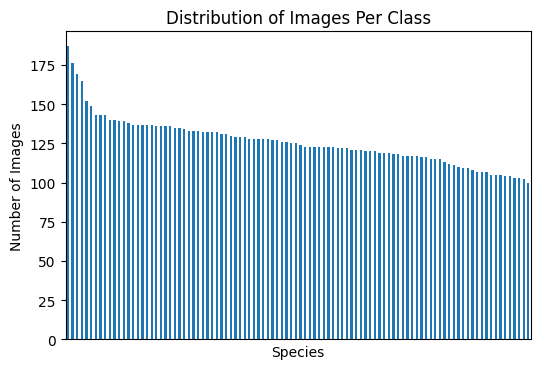
\includegraphics[width=0.5\linewidth]{imgs/classdist.png}
  \caption{Distribution of species in training dataset}
  \label{fig:classdist}
\end{figure}
% IMAGE SIZES
Furthermore, while each image was exactly 224x224x3 pixels (since they were RGB), we noticed a large variation in the information within images. More saturated images had a higher file size while simpler images (for example, white backgrounds) had lower file sizes. The largest pictures contained 50kB of data, and the smallest contained 9kB, while most of the images contained 20 to 30 kB, as shown in the plot below:
\begin{figure} [H]
  \centering
  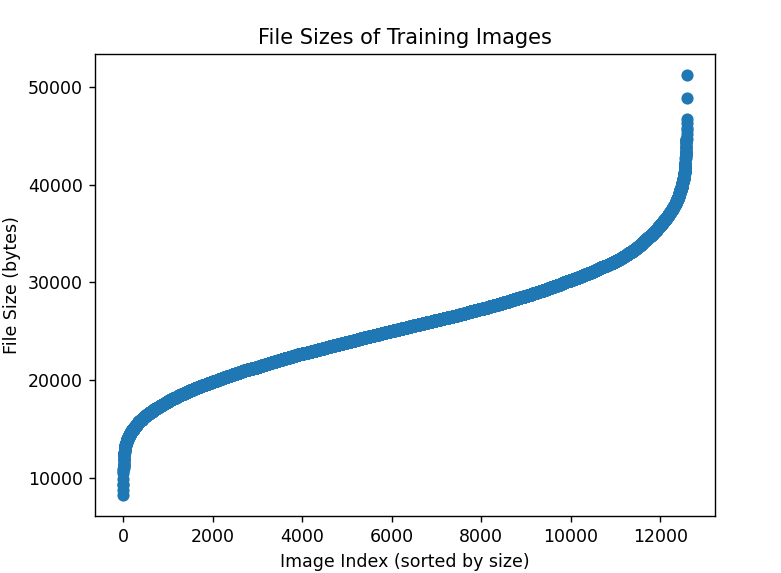
\includegraphics[width=0.5\linewidth]{imgs/imagefilesizedist.png}
  \caption{Distribution of image file sizes}
  \label{fig:imagefilesizedist}
\end{figure}

% VISUAL VARIABILITY
In terms of visual variability, we noticed two broad categories of images: insects in a nature scene, or insects in an expository position (typically a white background, fully open wings, and front-facing). Before doing any work, we hypothesized that the exposition-pose images would be generally easier to classify due to the obvious location and clarity of the subject, while natural images could be potentially difficult due to flowers, grass, and other objects in the photograph other than the subject. For example, consider the following examples:
\begin{figure}[htbp]

  \centering
  \begin{subfigure}[b]{0.3\textwidth}
    \centering
    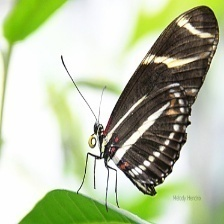
\includegraphics[width=\textwidth]{imgs/test_000999.jpg}
    \caption{An overexposed image, potentially hard to classify (\texttt{test\textunderscore 000999.jpg}).}
  \end{subfigure}
  \hfill
  \begin{subfigure}[b]{0.3\textwidth}
    \centering
    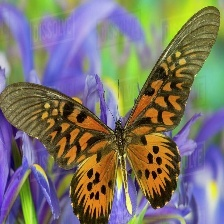
\includegraphics[width=\textwidth]{imgs/train_000199.jpg}
    \caption{A saturated image with flowers, potentially hard to classify (\texttt{train\textunderscore000199.jpg}).}
    \label{fig:middle}
  \end{subfigure}
  \hfill % Adds horizontal space between images
  % --- Third Subfigure ---
  \begin{subfigure}[b]{0.3\textwidth}
    \centering
    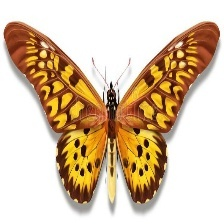
\includegraphics[width=\textwidth]{imgs/train_000187.jpg}
    \caption{An image with a clear exposition pose (clear subject, white background), likely easier to classify (\texttt{train\textunderscore000187.jpg}).}
    \label{fig:right}
  \end{subfigure}
  \label{fig:image_quality_comparison}
\end{figure}

\todo{the following paragraph is sketchy}
The exposition pose is the easiest one in terms of preprocessing (as our background removal packages excel at removing single colored backgrounds). Meanwhile, the natural ones posed a bigger challenge, as some pictures were overexposed (e.g. test\textunderscore image 00999), some were on top of flowers (e.g. train\textunderscore image 000199), which made edge detection harder. Also, we have realized that \textbf{color} and \textbf{wing shape} were the most drastic differentiators between two species of butterflies, so we incorporated the intuition we gained from those differences into the approaches we used in the preprocessing stage of our data.

\subsection{How we split the dataset for training and validation}
A common technique to ensure that we can correctly evaluate our model's performance and tune hyperparameters accordingly is to train the model on a training set and, evaluate it on a validation set. To reduce biases caused by the particular choice of the training/validation split, we also used k-fold cross validation (with k=5), in which we repeat the training/validation process 5 times with different splits and average the results to get a more stable estimate of our model's performance. We chose k=5 because we used the typical 80/20 train/validation split (80\% of the data for training and 20\% for validation) to maximize the number of images we can use for training while still having a good amount of data for validation; with that split, 5 folds would allow us to use all of our data for training and validation across the different folds.

\todo{reconsider this following part}
We chose this approach to partitioning the data because it has been empirically shown to excel in independent and identically distributed (i.i.d.) datasets with dozens of classes, but later, we also considered the following additions to our split:
\begin{enumerate}
  \item Since the butterfly data is not fully i.i.d because of the general appearance of the dataset we described above, and also we have relatively few images per species in the dataset, we can first ensure that each species is evenly weighted in the train/validation sets before training (by adding a term to account for how represented in the dataset each species is).
  \item Since we found out that some images were \textbf{exposed}, and some were \textbf{natural}, we can \textbf{tag the images accordingly and ensure that both are represented in the train/validation sets before training}.
  \item Another idea we found out that performed relatively well compared to naive approaches was training and validating the classifier was to use all data both to train and validate the model, but we thought that in relatively small per-class image numbers like our dataset, this would lead to overfitting; so we did not go into this approach.
\end{enumerate}

\section{Preprocessing of Data and Design Choices}
\subsection{Preprocessing pipeline applied to data before training}
We chose to apply different preprocessing pipelines to our different model architectures, as they have different requirements and are affected differently by the preprocessing steps.
% For example, the CNN model is more robust to noise and can learn features from raw data, while the SVM model is more sensitive to noise and requires more careful feature engineering. Hence, we applied a more complex and aggressive preprocessing pipeline to our CNN model, while we applied a simpler and more targeted preprocessing pipeline to our SVM model. \par

We started the preprocessing our data by resizing the images to 224x224 for our CNN model, 64x64 for SVM and converted them to NumPy/OpenCV arrays, which ensures that the sizes are standardized and makes conversion to/from data vectors/matrices easier, helping us produce a cleaner pipeline.
\subsubsection{Preprocessing for the CNN Classifier}
All of the transforms we used in our CNN pipelines were from the \texttt{torchvision.transforms} package, and we applied the following steps in our training pipeline:
\begin{enumerate}
  \item \texttt{ToImage()}: convert the initial 224x224x3 image vector to a PyTorch image tensor, which allowed us to utilize CUDA and improve training/prediction speed.
  \item \texttt{Resize(224 * 1.1)}: upscale the image tensor to about 245 pixels to create some room for randomness and thus help prevent overfitting to exact framings of a picture. (Professor Baraniuk demonstrated similar methods in class.)
  \item \texttt{RandomCrop(224)}: randomly crop the image to its original size (224x224), to force our model to learn to identify an object ``anywhere'' in the image, not just in the center.
  \item \texttt{RandomHorizontalFlip(p=0.5)}: since butterflies/moths are often symmetrically shaped, sometimes horizontally flip the image to prevent the model from having a bias toward left/right facing butterflies.
  \item \texttt{RandomRotation(degrees=10)}: a butterfly/moth can also be arbitrarily oriented, so randomly rotate the image anywhere from -10\degree \ to 10\degree \  to prevent the model from overfitting to the vertical orientations of our butterflies.
  \item \texttt{RandomAffine(degrees=0, translate=(0.1, 0.1))}: since the butterfly/moth can also be arbitrarily translated in the image, randomly translate the image by up to 10\% of its size vertically and horizontally to prevent the model from overfitting to the centered position of our butterflies (for example, in the exposition pose images like figure \ref{fig:right}).
  \item \texttt{RandAugment(ops=2, magnitude=10)}: beyond simple effects like rotations, translations, and reflections, the RandAugment augmentation method utilizes other augmentations that we did not explicitly code our pipeline for. We felt this could especially be useful for further expand the variability of our dataset and thus encourage the model to learn truly useful features.
  \item \texttt{ToDtype(torch.float32, scale=True)}: convert the pixel values to floats between 0.0 and 1.0, which is a more stable input range for our model to learn from, especially with ReLU activations.
  \item\texttt{ColorJitter(brightness=0.1, contrast=0.1, saturation=0.1, hue=0.02)}: we wanted our model to tolerate and learn different shades of a colored butterfly/genetic variations/dirt etc., but not too much since butterflies are mainly distinguished by their color, so apply a small random variation to the hue, saturation, saturation, and contrast of the image.
  \item  \texttt{Normalize(mean=(0.5, 0.5, 0.5), std=(0.5, 0.5, 0.5))}: center and normalize pixel values to ensure that the input data works well with ReLU steps in our CNN and that the training produces more stable gradients.

For our validation and test pipeline, we only convert the data to a Pytorch image tensor, ensure the image is 224x224x3, center and normalize, and convert to a float tensor. We do this because all the augmentation steps described above are useful in training the model, but we want consistent/stable validation, so we decided not to apply those preprocessing steps to our validation/test sets.
\end{enumerate}

\subsubsection{Preprocessing for HOG+RBF SVM} \todo{review this for accuracy}
\begin{enumerate}
  \item We used a smaller image size here (64x64), since we were not be able to parallelize because of the CPU-heavy inefficient nature of scikit-learn SVM algorithms, even with the addition of PCA.
  \item We also did a horizontal flip here using \texttt{np.fliplr()}, exploiting the symmetry of butterflies, and preventing our model from overfitting to left/right facing orientations.
  \item We then used a HOG-based edge/feature detector, which is a more modern and robust edge detection approach to the ones we learned in the class (like SIFT), using the method \texttt{hog()}. It essentially extracts edges, textures, and other shapes of the picture by computing gradients and comparing their directions. This was because the wing shapes play a huge role in differentiating butterflies, as we observed from our dataset.
  \item But one thing we skipped over when talking about HOG above was, it \textbf{skips coloring differences}. And as we mentioned, colors also play a huge role in differentiating butterflies, so we used histograms using \texttt{np.histogram(bins=32)} to count the red, green, and blue pixel intensities into 32 bins to append 96 features hinting about the color of our butterfly to our data vectors. This way, our model can differentiate between butterflies much more accurately.
  \item To avoid brightness/natural noise in colors, just like in the CNN but with a slightly different approach, we normalized our color histogram values so that the color features are actually comparable between pictures.
  \item We then unsurprisingly concatenated the HOG features with the color features by appending the color histograms to the HOG-based data vectors.
  \item After that, we applied the \textbf{most important preprocessing step in the SVM pipeline}, which was to normalize and center all of our data vectors, because SVM (especially with RBF kernel) can be extremely sensitive to disproportionate deviations in features.
  \item Finally, since HOG usually produces very large data vectors, we applied PCA to project all our data vectors onto the first $n$ eigenvectors that would capture 95\% of the variance so that both training and validation speed improve.
  \item \textbf{The validation/test pipeline was the exact same except that we did not flip the images, which would just introduce randomness into prediction. We wanted our prediction to be predictable.}

    \subsection{Background removal}
    We hypothesized that, due to the extra background information in the natural images (e.g. flowers and grass), a model could potentially perform better if we removed that background information and gave the model only subjects to learn. In other words, we thought that converting all images into ``exposition pose'' (subject on plain background) would improve our classifier's accuracy. This segmentation task itself proved to be challenging, and we tried a few methods with OpenCV functions, the most effective of which utilizes the GrabCut image segmentation algorithm using a full-image initial bounding box as well as morphological erosion and dilation operations. After trying different user-chosen parameters with the GrabCut algorithm, This was generally successful at isolating the subjects, but sometimes removed too much from the subject or did not remove enough. Consider the examples of the original image and the background-removed image in Figure \ref{fig:background_removal_comparison} below:
    \begin{figure*}[htbp]
      \centering
      \begin{subfigure}[b]{0.475\textwidth}
        \centering
        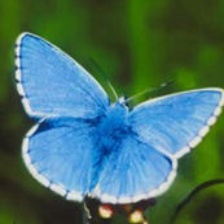
\includegraphics[width=\textwidth]{imgs/test_000003_orig.jpg}
        \caption{\texttt{test \textunderscore00003.jpg}, original.}
      \end{subfigure}
      \hfill
      \begin{subfigure}[b]{0.475\textwidth}
        \centering
        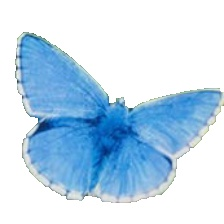
\includegraphics[width=\textwidth]{imgs/test_000003_crop.jpg}
        \caption{\texttt{test \textunderscore00003.jpg}, cropped; near-perfect segmentation of the subject and background.}
      \end{subfigure}
      \vskip\baselineskip
      \begin{subfigure}[b]{0.475\textwidth}
        \centering
        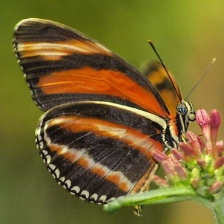
\includegraphics[width=\textwidth]{imgs/test_000081_orig.jpg}
        \caption{\texttt{test \textunderscore00081.jpg}, original}
      \end{subfigure}
      \hfill
      \begin{subfigure}[b]{0.475\textwidth}
        \centering
        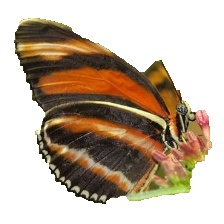
\includegraphics[width=\textwidth]{imgs/test_000081_crop.jpg}
        \caption{\texttt{test \textunderscore00081.jpg}, cropped; failure to fully remove the flowers.}
      \end{subfigure}
      \caption{Original images and background-removed images}
      \label{fig:background_removal_comparison}
    \end{figure*}

    This technique improved the accuracy of our KNN+SIFT model a little, but surprisingly led to worse performance in our more complex CNN model. Presumably this occurs because it removes noise from the data, which KNN is more vulnerable to but a CNN can learn.\todo{review this statement}
\end{enumerate}

\subsection{Comparison of the used preprocessing pipelines} \todo{review}
\subsubsection{Feature extraction}
\begin{enumerate}
  \item \textbf{In our HOG+SVM model,} we deterministically computed edges using HOG and color distribution using histograms. This gave us a fixed representation of each image.
  \item \textbf{In our CNN model,} we let the neural network 'learn' the features by detecting the edges in the early layers, the textures in the middle layers, the object parts in the deeper layers. This gave us a more adaptive representation of each image, provably superior to HOG+SVM since if that fixed representation misses something about the butterfly, HOG cannot recover, while CNN can learn more about the useful features by introducing layers.
\end{enumerate}
\subsubsection{Data augmentation}
\begin{enumerate}
  \item \textbf{In our HOG+SVM model,} we only did a horizontal flip on the images. This is because edges do not change much by color/lighting changes and since HOG is a much lower capacity model (compared to neural networks), too much augmentation can drastically reduce model accuracy rather than improving it.
  \item \textbf{In our CNN model,} we applied a bunch of different random augmentations on our data (as mentioned above), ranging from cropping it to changing the contrasts. This is because even though CNNs learn the features of an image well, they might sometimes learn them \textit{too well}. We need a lot of variation in augmentation to prevent overfitting to the data, especially in a dataset like this where in many of the images the object (butterfly) is relatively in the center of the picture.
\end{enumerate}
\subsubsection{Local spatial information}
\begin{enumerate}
  \item \textbf{In our HOG+SVM model,} the preprocessing steps (HOG+color histograms) do not really tell us about the locations of a color in an image, which means the loses the spatial information while training. In non-neural-network pipelines, especially a HOG-based SVM, this is inevitable because HOG cannot differentiate colors, only shape and separate preprocessing approaches like color histograms only differentiate color, not shape.
  \item \textbf{In our CNN model,} we use \textit{convolutions} to keep and propagate the information on which color appears where in the image. Unlike the SVM approach, this helps us pinpoint what each part of a butterfly is colored and how it differentiates it from the others.
\end{enumerate}
\subsubsection{Normalization}
\begin{enumerate}
  \item \textbf{In our HOG+SVM model,} we normalize the features of our data \textit{after} we are done with extracting the features. This is because HOG representations make the RBF kernel SVM extremely vulnerable to small disproportionate variations in features.
  \item \textbf{In our CNN model,} we normalize the pixels of our data \textit{before} we start learning the features. This is because the CNN needs a stable input range to learn the features and is much more stable to small variations compared to other approaches like the SVM.
\end{enumerate}
\subsubsection{Dimensionality reduction}
\begin{enumerate}
  \item \textbf{In our HOG+SVM model,} we apply PCA on our data vectors to capture 0.95 of the variance, because training and testing the SVM is a sequential, CPU-heavy process.
  \item \textbf{In our CNN model,} we do not externally apply any dimensionality reduction but let the layers of our neural network handle it. The pooling, convolutions, and compression inside the hidden layers do the 'dimensionality reduction' for us. Moreover, CNN training is parallelizable with CUDA in nature, so it is much more efficient with more features.
\end{enumerate}

\section{Models Considered}
\subsection{ResNet CNN}
\subsubsection{Why we chose to try it}
We have read some articles online that the peak image classification accuracies in diverse datasets like Caltech 101 were around 70-80\% without the use of convolutional neural networks (CNNs)\cite{svmacc}, and that CNNs broke this wall and reached around 90-99\% accuracy with ease.\cite{imagenet}\cite{Zabir_Fazira_Ibrahim_Sabri_2018} Also, the project descriptions explicitly states that one of our model choices shouldn't be a neural network, which suggested to us that a neural network might perform quite well. In addition, CNNs are well-known architectures for approaching image classification problems like MNIST digit recognition or the ImageNet dataset.
\subsubsection{Algorithm/Workflow} \todo{review}
A convolutional neural network performs similarly to how a human brain is thought to visually recognize an image, and it has a simple pipeline once the algorithm is understood well. It works by passing the inputs through a variety of hidden layers before finally predicting class probabilities with a ``logistic regression'' output layer. Moreover, it uses matrix convolution rather than explicit vector/array multiplication to significantly reduce the number of model parameters, allowing us to deepen the model without significantly decreased performance or vanishing gradients in the backpropagation process. The workflow is as follows:
\begin{enumerate}
  \item We pass preprocessed images to the first layer.
  \item The first layer, we first perform \textbf{feature extraction} on the input using 2-dimensional convolutions to learn the edges and color gradients.
  \item We then downsample the data using max-pooling so that we only keep the strongest indicators/features.
  \item Then, we pass them to the middle hidden layers, which build up increasingly complex patterns from the features using an arbitrary/tuneable variety of approaches where we will discuss in the \textit{How Each Model Was Trained} section.
  \item After that, we perform a spatial compression using average-pooling, which removes the spatial dimension to only leave the information about 'how strongly each feature was present in the data'.
  \item Finally, we flatten our data to a vector that is the size of the number of our classes, similarly to how one would do 'logistic regression' in the final layer of our network.
  \item Now that we are ready to score our vector, we optimize over the cross-entropy loss function we learned in class, with a good optimization algorithm (adamW, for example).
  \item We then backpropagate the gradients we get from our optimization algorithm, and update the weights of our model.
  \item We repeat this process until our loss converges, or until we hit the maximum number of epochs we set.
\end{enumerate}
\subsubsection{Design choices that affect the model}
\begin{enumerate}
  \item \textbf{Amount of feature complexity through layers:} We want to gradually increase feature complexity through the layers of our neural network, so in the first layers, we want to learn simpler things like edges and color; but as we go deeper in the network, we also want to learn more specific things like the markings on a butterfly. So, we need to gradually increase feature sizes and complexity of the operations we perform in the layers and residual blocks. (for example, start with just linear layer + relu, and continue with multiple layers of relu + 1-norm normalization)
  \item \textbf{How much to reduce image size as we process it:} We want easier to analyze, smaller representations of an image that preserves what is present in the image correctly. But we also do not want to lose the actual features of an image that differentiate it from the others. So, we need to choose the step by step scaling accordingly.
  \item \textbf{The number of residual blocks and layers we use:} We want a model that both accurately detects objects (butterflies) and has high performance in training, validation and testing, also speed-wise. Therefore, we need to be careful about adjusting how many features each residual block introduces into the data, and how many of the layers/blocks we have. Too many layers and residual blocks can impact performance while introducing marginal accuracy/maybe causing overfitting, but too few can cause the model to underfit or become unstable.
  \item \textbf{Learning rate: scheduled or constant?} A learning rate too large can cause the model to become very unstable or overshoot the optimum, but one too slow can negatively impact the learning performance of our model. Hence, we should decide on what the initial learning rate is, and if we should decay the learning rate or not.
  \item \textbf{How to decay the model weights over time:} Too large model weights can cause the model to overfit, and too much decay in the weights can cause the model to underfit. We also need to implement a schedule on decaying the weights of our model to keep it consistent.
  \item \textbf{What to choose the batch size:} Since the optimization methods we use are usually based on batch optimization (like adamW), we need to choose a batch size that is enough to produce a stable training process, but one that is not too large so that the training stays fast.
  \item \textbf{What to choose the loss function and optimizer:} Like in many other problems, the cross-entropy loss function is generally unmatched in its success here. So, we do not regard it as that flexible of a choice but still wanted to include it here. Coming to the optimization algorithm, we need an optimization algorithm that both incorporates fast early learning, and later fine-tuning. Moreover, it would help us if our optimizer decayed the weights/scheduled the learning for us. (Yes, we are hinting at adamW, adaptive moment estimation with weight decay)
  \item \textbf{The preprocessing steps before the data is input:} \textbf{This is in fact the most important part as CNNs depend heavily on their input, just like most classification models. We have already discussed these choices and the steps we used in the previous section.}
\end{enumerate}

\subsubsection{Course concepts used in the model}
\begin{enumerate}
  \item \textbf{Supervised learning/Classification:} Obviously, the CNN we trained here is effectively a supervised learning model where inputs are images (data) with labels and the outputs are a discrete number of classes. Hence, this is effectively a classification problem.
  \item \textbf{Feature engineering and learning:} Our CNN learns the features of the data by applying convolution layers and residual blocks.
  \item \textbf{Optimization/OR:} We have a convex loss function that is called cross-entropy (log-loss), and we use an optimization algorithm based on \textit{Gradient Descent} that is called adamW.
  \item \textbf{Linear algebra background:} Since we are working with matrices, tensor operations, convolutional layers, max-pooling, and backpropagation of gradients; we are especially counting on the concepts we learned from Multivariate Calculus and Linear Algebra.
\end{enumerate}
\subsubsection{Loss function of the model and how it is optimized}
As we mentioned, our model uses the cross-entropy loss, otherwise known as log-loss; and uses adamW to optimize it. The cross-entropy loss is derived from Maximum Likelihood Estimation (MLE) of logistic regression, and it has two terms, where one activates and the other deactivates. It is also convex, and hence optimizeable by gradient descent-based algorithms. AdamW is a fairly new algorithm that uses 'adaptive moment estimation' and 'weight decaying', in which the 'moments' are closely related to gradients in gradient descent; and weight decaying is just a smart way of steering the model away from underfitting to more previous data in the training procedure.
\subsection{Model 2: HOG+RBF Kernel SVM}
\subsubsection{Why we chose to try it}
It was given to as our Homework 7 in the course. The homework problem was about implementing a Kernel SVM using the Gaussian (RBF) kernel and fitting it to the butterfly data we have at hand and finally, submitting it to Kaggle. We also chose this model to have a strong contender for the required 'non-neural-network based model' in the final project. We read some articles online that suggested with the right training regimen and preprocessing (HOG), kernel SVMs can achieve accuracies as high as 70\% in multi-class classification problems similar to our dataset (like Caltech 101).
\subsubsection{Algorithm/Workflow}
Support vector machines (SVMs) are essentially classifiers that fit an arbitary-dimensional hyperplane to separate the data points. But moreover, they try to 'regularize' that hyperplane by actually fitting a hyper-slab; achieving that by maximizing the margin of the hyperplane (thickness of the slab). This ensures that the classification model is more stable for the future data to come, even if it trades off some accuracy for the training data while doing so. And most of the time, the data we are working with is not 'linearly' separable in $d$ dimensions, so we use one of the most powerful kernels that we can apply the kernel trick on, which is the RBF kernel; because any data is 'linearly' separable in $\infty$ dimensions, which the RBF kernel maps the data to. With the combination of these two approaches, the Kernel SVM works as follows:
\begin{enumerate}
  \item We assume all the preprocessing steps (up until PCA) have been applied to the data before it is input to the Kernel SVM for training.
  \item We first use the Gaussian (RBF) kernel to map our data to 'infinite' dimensions.
  \item We then using the kernel trick, optimize our loss function (which is the '1/margin'-penalized hinge-loss and train the SVM.
    \item While training, depending on $\lambda \sim 1/C$, we let some of the points be misclassified, for which we call them our \textbf{support vectors}.
    \item We then use the support vectors to implement our decision function, in which the decision function looks like as follows:
      \begin{center}
        $f(\mathbf{x}) = \sum_{i \in SV} \alpha_i y_i K(\mathbf{x}_i, \mathbf{x}) + b$
      \end{center}
    \item Depending on the decision function value, we predict the class of the validation/test set. i.e.:
      \begin{center}
        $\hat{y} = \arg\max_{k} \; f_k(\mathbf{x})$
      \end{center}
  \end{enumerate}
  \subsubsection{Design choices that affect the model}
  \begin{enumerate}
    \item \textbf{Kernel choice:} We need a kernel that has enough dimensionality to get us a linearly separable transformation, but also one that prevents overfitting and is stable. RBF kernel is known to have both of those features. For example, the sigmoid(tanh) kernel is known to be unstable even though it also maps the data to 'infinite' dimensions; and the polynomial kernels are known to overfit/underfit easily to complex datasets.
    \item \textbf{Regularization parameter $C$:} Do we want higher bias, lower variance (higher $C$) in our hyper-slab, or vice versa (lower $C$)? This can drastically change our prediction accuracy, and is a good 'knob' to adjust to get higher prediction accuracy/lower overfitting levels.
    \item \textbf{RBF exponentiation scaler $\gamma$:} If we increase this value, even the slightest spatial local adjustments between data can affect our classifier, which can lead to overfitting. However, if we decrease this value, our classifier may underfit. We also need to pay attention to this 'knob' to get a good classifier.
    \item \textbf{Just like the CNN model, the preprocessing steps before the data is input are the most important of the design choices we can make, as most of the work we have done on training this classifier was actually in the preprocessing part (HOG+PCA). If the input data does not provide a well representation of the images we are trying to classify, what good is optimizing over it?}
    \item \textbf{Course concepts used in the model}
      \begin{enumerate}
        \item \textbf{Supervised learning/Classifiaction:} Similarly to the CNN model, we are essentially doing supervised learning here, and the problem is a classification problem.
        \item \textbf{Optimization/OR:} We are solving a convex optimization problem by minimizing hinge-loss while maximizing margin in the SVM training. We are using a variant of (stochastic) gradient descent to solve this problem, hence we are relying on our optimization principles.
        \item \textbf{Unsupervised learning/PCA:} This is only used in the preprocessing step to make our training process smoother and faster.
        \item \textbf{Feature engineering and learning/HOG+color histograms:} While this is also only used in the preprocessing step, this part is very crucial to our model and we need a good manual design of features to accurately represent our data.
        \item \textbf{Kernel methods/Kernel trick:} This is the core method to make our data vectors linearly separable, and we achieve this using the RBF kernel + the kernel trick.
        \item \textbf{Linear algebra background:} We are also working with matrices and vector operations here both in the preprocessing of the data and the training of the model. We also use gradients in optimization, hence Multivariate Calculus and Linear Algebra also heavily appear in this model.
      \end{enumerate}
  \end{enumerate}
  \subsection{Model 3: KNN + SIFT}
  When we started looking for filters for our image processing step, we noticed that SIFT reduced each image from nearly tens of thousands of parameters down to 196. Then, as we remembered that the one of the main issues with KNN was the time complexity we thought that given the reduced data set size, it would be more manageable for it.\\
  Furthermore, as the points of interest are scale and rotation invariant, this improves KNN ability to deal with rotated pictures (which was a severe issue as it changes almost all the pixels around).\\
  In the end, our performance was at most around 42 \% for this model. So, it was still not the best non-neural network based model (which was rather unfortunate, given this was our original model)\\
  We initially were considering other ways to improve our model. However, we ran into a few issues, the most important one is that SIFT does not account for any form of color, which is quite helpful for classifying butterflies. Moreover, when we started looking into other possible filters, almost all of them increased the image complexity- which made KNN very inefficient at classifying.
  Thus, given that the performance (at best around 40\%) was still considerably worse than the our simple first implementation of SVM, we ended up deciding not to proceed any further with this architecture.
  \section{Training Procedures}
  We describe the training and validation process of our models as implemented in our Python code in this section (PyTorch Lightning notebook \texttt{kfold\_clf.ipynb}, \texttt{svmkernel\_model.py}, and \texttt{sift\_knn\_classifier.py}). Preprocessing and data augmentation are already summarized in the previous sections; hence, here we focus on data splits, optimization, schedules, regularization, and how we trained each classifier.

  \subsection{Model 1: ResNet CNN (with PyTorch Lightning)}
  We used PyTorch Lightning to train our CNN classifier, as the library allowed us to streamline our code, as well as quickly iterate training the model with different hyperparameters and maintain comprehensive logging of the training process. The model architecture is based on ResNet-18, which has 18 layers with three structural changes compared to the ImageNet: the first convolution uses stride of 1 and padding of 1 (we downsample later compared to the usual ResNet architectures); the max-pooling stage is replaced by an identity mapping to preserve more fine-grained information; and the original fully connected layer is replaced by a two-part head dropout block with probability 0.4 followed by a linear mapping from 512 features to 100 classes (the output number of classes). The model applies dropout only at the head and not inside the residual blocks.
  \begin{enumerate}
  \item\textbf{Data partitioning.} We use \texttt{sklearn.model\_selection.StratifiedKFold} with shuffling, \texttt{random\_state}=42 for reproducibility, and \texttt{n\_splits}=6 for 6-fold cross validation (even though we mentioned 5-fold above, averaging across our 6-fold results proved marginally superior in our experiments). This way, we train and test our classifier by averaging out the parameters learned from the whole dataset, yielding a more stable training and test regimen.
  \item\textbf{Mini-batch training.} For each fold in our training and validation process, \texttt{ImageDataset} maps CSV rows to integer labels via a fixed alphabetical ordering of class names. The training dataloader uses a batch size of 32, random shuffling, \texttt{num\_workers}=4 for faster training/prediction, and \texttt{pin\_memory=True} for increased performance. Validation and test prediction loaders use the non-augmented preprocessing pipeline aforementioned since they should make predictions on the raw data; and the test \texttt{DataLoader} uses a batch size of 1 to make predictions sequentially.
  \item\textbf{Class imbalance in the loss.} Before we fit a fold, we compute class frequencies on the fold's training frame. We set the class-weights proportional to the inverse frequency (total count divided by class count, scaled by the number of classes) and pass them into \texttt{nn.CrossEntropyLoss} as tensor weights. This reweights the softmax cross-entropy so we balance \todo{what does this mean?}exploration and exploitation by making species with less number of samples contribute relatively more to the gradients.
  \item\textbf{Loss, label smoothing, and optimization.} The training configuration sets label smoothing to 0.1 combined with the weighted cross-entropy approach we discussed above. This replaces one-hot truth label vectors by smoother versions, ideally improving the model's generalizability and accuracy. \todo{Explain why use AdamW, move details from below up here} Our optimizer is AdamW with learning rate $3\times10^{-3}$ and weight decay of $10^{-2}$. \todo{Discuss how we also tried CosineAnnealingWarmRestarts and ReduceLROnPlateau but the most significant change to our accuracy came from using a small initial learning rate and our ResNet architecture} A cosine annealing scheduler (\texttt{CosineAnnealingLR}) runs through the maximum number of epochs with \texttt{T\_max = 100}, stepping once per epoch. We also enable mixed-precision training when supported (\texttt{16-mixed}) for increased performance and better memory complexity; and we also set \texttt{torch.set\_float32\_matmul\_precision('medium')} for the Tensor Core behavior on the utilized NVIDIA GPUs to help speed up the training process.
  \item\textbf{Stopping, checkpoints, and logging.} We use early stopping in our training process \texttt{val\_accuracy} with a patience of 12 epochs to detect convergence. The \texttt{ModelCheckpoint} keeps the top three checkpoints by validation accuracy, saves the last checkpoint in the file \texttt{last.ckpt}, and stores the files under a run directory for each fold of the training process. We use a learning rate monitor and a progress bar for easier analysis of checkpoint convergence; and we log the metrics with \texttt{CSVLogger}. We can resume the training from the last checkpoint whenever \texttt{RESUME\_FROM\_LAST\_CHECKPOINT} is true, making the training progress more flexible.
  \item\textbf{Ensembling across folds.} After training each fold, we load the checkpoints and either average the logits across folds or take a per-sample majority vote among the argmax predictions from each fold. After that, we map the indices back to species names for submission. We use this approach to exploit the diversity of our dataset and have a more stable classifier since it has been empirically shown in studies that ensembling can help increase accuracy while also improving overfitting.\cite{8539396}
\end{enumerate}
  \subsection{Model 2: HOG + RBF kernel SVM (\texttt{svmkernel\_model.py})}
  Unlike our ResNet CNN model, we do not use $k$-fold cross validation in this model. However, if we wanted to further improve this model, we might want to use it; as having observed its high accuracy in our CNN classifier. We still map the labels to integers (with \texttt{LabelEncoder} this time). A single data split (\texttt{train\_test\_split}, 80\% train / 20\% test, \texttt{random\_state}=42 for reproducibility, stratified on encoded targets) defines our training and validation sets as it is a common approach to set the split proportions to 80/20.
  \begin{enumerate}
  \item\textbf{Feature construction and fitting order.} For each training row, features are extracted twice when \texttt{flip=True} is used on the second pass, hence the training set effectively doubles in size (original plus mirrored vectors - reason explained in preprocessing section). Like our other models, we only use the non-augmented data for validation. After stacking the vectors, we fit \texttt{StandardScaler} on the training matrix and apply it to both train and test feature matrices. We then do PCA on the training data to improve performance with \texttt{n\_components=0.95} (retain 95\% of variance), and the same PCA transforms validation features, also to improve performance. We fit the scaler before PCA to improve accuracy on the validation data.
  \item\textbf{SVM training.} We use the scikit-learn implementation of the SVM classifier \texttt{sklearn.svm.SVC} with the Gaussian Kernel \texttt{kernel='rbf'}, \texttt{cache\_size=5000} MB for performance, and \texttt{random\_state}=42 for reproducibility. Hyperparameters $C$ and $\gamma$ are left at their library defaults (so $C=1$ and $\gamma$ uses the ``scale'' heuristic). We fit the model on our full PCA-reduced, augmented training set in one batch solve; and report the validation accuracy metrics with \texttt{score} on the held-out 20\% of the data.
  \end{enumerate}

  \subsection{Model 3: KNN + SIFT (\texttt{sift\_knn\_classifier.py})}
  We have left this pipeline light using mostly built-in and already implemented packages to focus more on more promising approaches, as this is more of an experiment because Prof. Baraniuk told in class that K-NN performs well in general even though the complexity is high. We run OpenCV's SIFT implementation (\texttt{cv.SIFT\_create}) on the grayscale images we read from the dataset. We then standardize the variable length SIFT output to vectors of fixed length: we concatenate the mean and standard deviation of all 128 rows to the data, giving 256 features per image. If no keypoints or descriptors are returned, we substitute that with a zero vector - but this rarely happens in our dataset from our observations after fitting the model.
  \begin{enumerate}
  \item\textbf{Training subset and $k$-NN.} To reduce runtime, we only use every fifth row of \texttt{train.csv}. We skip (\texttt{idx \% sample\_rate != 0} with \texttt{sample\_rate}=5), so, roughly 20\% of labeled data participate in fitting. This is to increase performance since as we mentioned, KNN is a slow classifier with high time complexity. We standardize the features with \texttt{StandardScaler} fit on that subset. We use the \texttt{KNeighborsClassifier} with the default $k=5$ neighbors and Euclidean distance metric. We do not perform an explicitly training/test split on this dataset to keep complexity of the model low, and performance high.
  \end{enumerate}

  \section{Quantitative Comparison of the Models}
  \subsection{Model 1: Neural Network}
  \subsubsection{Training performance and robustness}
  \textbf{TODO: Explain how RELATIVELY easy it was to train the model with the data at hand.}

  Although training the ResNet was the most computationally expensive part of the entire project, it was still a relatively easy process. As the architecture is extremely flexible in learning patterns, and we utilized different packages to optimize for the hyperparameters (mention a few ones, e.g. ADAM, or the one Rishabh used for early stopping), we did not have to account so much for particular aspects of our data (at least not compared to when we implemented the other methods, that lead us to HOG and SIFT).

  \subsubsection{Validation performance and accuracy}
  \textbf{TODO: Provide data on how accurately the model validated the validation set.}
  \subsubsection{Kaggle/test accuracy of the model}
  As seen in our Kaggle submission, we managed to obtain an extremely high prediction accuracy, which was comparable to the one from our test dataset.
  \textbf{TODO: Elaborate on the Kaggle accuracy of the model, and how it compares to the validation accuracy.}
  \subsubsection{Relative strengths and weaknesses of the model}
  \textbf{TODO: Based on how the model quantitatively compares to the other models in terms of performance, also based on the correspondence between its validation and test performance, elaborate on the strengths and weaknesses of the model. For example, a strength can be validation and test accuracies both being high, implying less overfitting. A weakness can be long training times and requirement of precise tuning.}
  \subsection{Model 2: Whatever}
  do the same thing as above

  \section{Overfitting and Generalization Analysis}
  \textbf{TODO: Describe the instances where your models overfit/underfit, by first stating which model it was, and elaborate on what caused it. Then discuss strategies you resorted to, to overcome that over/underfitting. You might find it useful to explain overfitting/underfitting using the validation/test accuracy discrepancies of the model stated above.}
  \subsection{Overfitting in Neural Network Model}
  \subsubsection{Evidence of overfitting}
  The main evidence of overfitting in our model, was that we had a training accuracy of over 99\%, and a validation accuracy of 93 \% (our final submission accuracy was somewhat higher, but we achieved that by using a voting model across our different data splits). So, this is the main trait of overfitting, improved performance on training set, which did not improve the actual model performance.

  \subsubsection{What may have caused it}
  As we have learned in class, because neural networks have such exceptionally large number of weights to classify. Thus, as expected, it manages to reduce the training data error significantly, even though it does not translate into actual improvements in the accuracy.

  \subsubsection{How we tried to overcome it}
  \textbf{TODO: Elaborate on what methods you used on mitigating the overfitting, and how well it mitigated it. If you were unable to improve, relate it to model complexity and task difficulty.}

  We reduced overfitting by doing early stop, using weight decay (i.e. a ridge penalty), and using dropout layers.
  % Someone double check

  \subsection{Underfitting in whatever}
  same argument.

  \section{Pipeline for the Final Submission}
  \textbf{TODO: Explain each process of an image's journey in the final submission pipeline, starting from its preprocessing up until how it's classified with a given label. HIGHLY RECOMMEND TO ADD A FLOWCHART OR A VISUAL DRAW.IO MODEL ETC HERE!}
  \subsection{Preprocessing of the image}
  \textbf{TODO: Briefly explain how a particular image is preprocessed in the final pipeline.}
  \subsection{Final model choice and its properties}
  \textbf{TODO: Briefly explain what model you chose for the final pipeline touching on the properties of the image that the model suits well.}
  \subsection{How the image trains the model}
  \textbf{TODO: Briefly explain how the image is used in the training process of the model, touching on exactly how it improves the optimization process}
  \subsection{How the model classifies the image}
  \textbf{TODO: Briefly explain how the model processes the image to label it.}

  % Someone can correct this.
  % keep in mind that they only asked us for th final pipeline, i.e. we only need to talk about Resnet

  \subsection{Flowchart}
  \begin{center}
    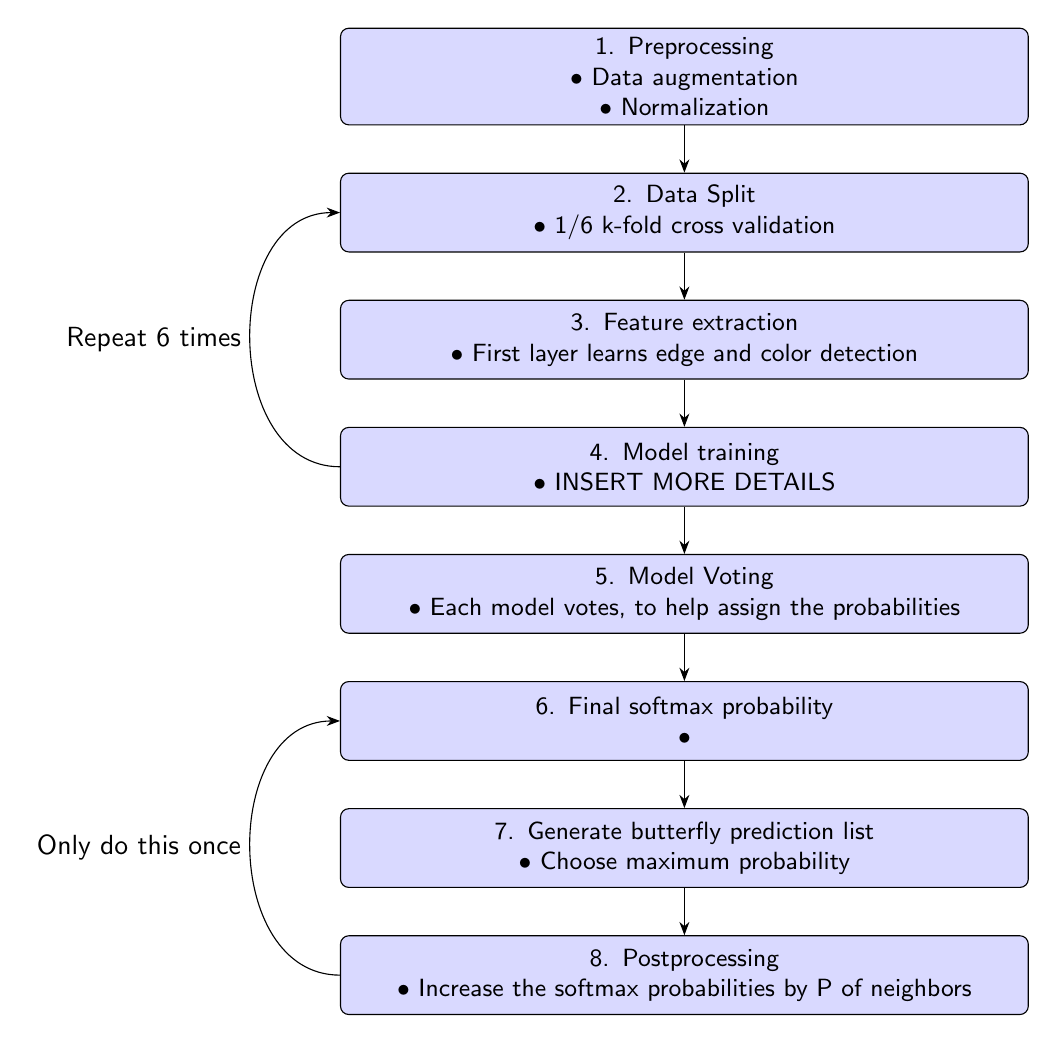
\begin{tikzpicture}[
        node distance=0.6cm,
        block/.style={
          rectangle,
          rounded corners=3pt,
          draw=black,
          fill=blue!15,
          text width=8.5cm,
          align=center,
          minimum height=1cm,
          font=\small
        },
        arrow/.style={
          -{Stealth[scale=1]},
          draw=black
        }
      ]

      % Nodes
      \node [block] (b1) {1. Preprocessing \\ $\bullet$ Data augmentation \\ $\bullet$ Normalization};
      \node [block, below=of b1] (b2) {2. Data Split \\ $\bullet$ 1/6 k-fold cross validation};
      \node [block, below=of b2] (b3) {3. Feature extraction \\ $\bullet$ First layer learns edge and color detection};
      \node [block, below=of b3] (b4) {4. Model training \\ $\bullet$ INSERT MORE DETAILS};
      %4. Data Split \\ $\bullet$ Train / Validation / Test
      \node [block, below=of b4] (b5) {5. Model Voting \\ $\bullet$ Each model votes, to help assign the probabilities};
      \node [block, below=of b5] (b6) {6. Final softmax probability \\ $\bullet$};
      \node [block, below=of b6] (b7) {7. Generate butterfly prediction list \\ $\bullet$ Choose maximum probability};
      \node [block, below=of b7] (b8) {8. Postprocessing \\ $\bullet$ Increase the softmax probabilities by P of neighbors};

      % Sequential Arrows
      \draw [arrow] (b1) -- (b2);
      \draw [arrow] (b2) -- (b3);
      \draw [arrow] (b3) -- (b4);
      \draw [arrow] (b4) -- (b5);
      \draw [arrow] (b5) -- (b6);
      \draw [arrow] (b6) -- (b7);
      \draw [arrow] (b7) -- (b8);

      % Feedback Arrow
      \draw [arrow] (b8.west) to[out=180, in=180, looseness=1.2] node[left] {Only do this once} (b6.west);
      \draw [arrow] (b4.west) to[out=180, in=180, looseness=1.2] node[left] {Repeat 6 times} (b2.west);

    \end{tikzpicture}
  \end{center}

  \section{``Post-Processing''}
  (Note for grader: we asked on Piazza whether this is a valid technique, and the instructor response said it was)\par
  After we looked at the test images, we noticed an odd pattern: there was significant cluttering of butterflies in sequential order. This makes sense, considering that if we were to look at a user feeding data into some form of database, they would probably in clusters- as someone might take multiple pictures of the same butterfly. Furthermore, it is expected that the classification would have some natural statistical biases, for example- we might expect that if a past butterfly is from a certain location, then other species in the same region would be more likely. Thus, it makes sense to also account for those patterns when creating a classifier. \par
  Hence, we altered our prediction pipeline. Once we had our predicted list of butterflies, we retroactively scaled the softmax probability vector by a (1- 2$P$) and added P (a tunable hyperparameter) to the probability of the neighboring butterflies. With that, we managed to achieve 99.8 \% accuracy on the test dataset. \par
  It is worth noting though that this also increases the chance of overfitting to the particular dataset that we were working with, if someone decided to shuffle the data the accuracy would then go down quite a lot; so, it is important to tune the P value.

  \section{Results and Conclusion}
  \subsection{Results of the project - what we learned}
  \textbf{TODO: Reflect on the overall results of the project and what new information you have learned.}

  \subsection{Comments on the final model's performance}
  \textbf{TODO: What do you think about how your final model performed in terms of performance and accuracy? Elaborate.}
  We were reasonably satisfied with the final performance of our models. In particular, the ResNet was quite good at predicting, an
  \subsection{What surprised us}
  \textbf{TODO: List all the things that were unexpected. They can be good, bad, or ugly.}
  We were surprised when looking at some of the misclassified butterflies. While the majority of them had some large visual variation (e.g. the wings were shown from the top, which has a very different visual aspect to the bottom of the butterfly, and looked like another species). However, there some classifications that seemed similar to the rest of the dataset, so we were surprised that they were misclassified (which goes to show, as discussed in class that Neural Networks can be sensitive to small changes, producing unpredictable errors).
  \subsection{What's new to come}

\AddToHook{cmd/section/before}{\clearpage}
%I made this into its own page
\bibliographystyle{plainnat}
\bibliography{references}
  \end{document}
